\documentclass[8pt,xcolor*pst]{beamer}
\input{packages-slides.tex}
\input{macro.tex}
\bibpunct{(}{)}{\phantom{ }; }{a}{,}{,}
%\bibpunct{(}{)}{\hspace{1.em}; }{a}{,}{,}

\makeatother

{\newtheorem{ndr1va}{\textbf{\textsc{Redaction note V.A.}}}[section]}

\newenvironment{ndrva}%
{%
\noindent\begin{ndr1va}\hrule\vspace{1em}%
}%
{%
\begin{flushright}%
\  \\
%\vspace{-1.5em}\ding{111}
\end{flushright}%
\vspace{-1.5em}\hrule
\end{ndr1va}%
}
\makeatletter

\newtheorem{remark1}{Remark}
\newenvironment{remark}%
{%
\noindent\begin{remark1}\hrule\vspace{1em}%
}%
{%
\begin{flushright}%
\  \\
%\vspace{-1.5em}\ding{111}
\end{flushright}%
\vspace{-1.5em}\hrule
\end{remark1}%
}
%%% Local Variables: 
%%% mode: latex
%%% TeX-master: t
%%% End: 

%hideothersubsections
%\usetheme[hideothersubsections,width=1.5cm]{Franck}
\usetheme[]{Franck}
%\useoutertheme[headline=empty]{miniframes}
\title{Automatic circuit equation formulation for non-smooth electrical circuits}
\author{Vincent Acary, Olivier Bonnefon, Pascal Denoyelle}
\date{February 07, 2008}
\institute{INRIA Rh\^one-Alpes}
%\includeonly{
%test
%}

\newcommand{\FontVince}[1]{{\usefont{T1}{pag}{m}{n}\fontsize{7.74pt}{7pt}\selectfont #1}}
\newcommand{\FontSmall}[1]{{\usefont{T1}{pag}{m}{n}\fontsize{7.74pt}{4pt}\selectfont #1}}
\begin{document}

\frame{\titlepage}
%\section{Outline}
\frame{\tableofcontents}%[pausesections]}
\section{Basics on circuit topology}
\frame
{
  \frametitle{Basics on circuit topology and analysis}

}

\frame
{
  \frametitle{Circuit branch}
\begin{figure}[h]
\centerline{
 \scalebox{0.4}{
    \input{Branch.pstex_t}
 }
}
\caption{Basic branch}
\end{figure}
A branch is described by a pair of branch variables: the tension $U_{a}$ and the current $I_{a}$.
Moreover, the Branch Constitutive Equation can be expressed in a general implicit form:
\begin{equation}\label{BCE}F(U_{a},I_{a},\frac{dU_{a}}{dt},\frac{dI_{a}}{dt},...)=0\end{equation}
Some examples with a resistor, a capacitor and a current source:
\[U_{a}=RI_{a} \qquad I_{a}=C\frac{dU_{a}}{dt} \qquad I_{a}=\alpha U_{b}\]
We will see the different forms of this relation.
  }

\frame
{
\newtheorem{kcl}{The Kirchhoff Current Law (KCL)}
\begin{kcl}
At any node in an electrical circuit where charge density is not changing in time, the sum of
currents flowing towards that node is equal to the sum of currents flowing away from that node.
\end{kcl}
\begin{figure}[h]
\centerline{
 \scalebox{0.35}{
    \input{SimpleCircuit.pstex_t}
 }
}
\end{figure}
With this example $N_n=2$, $N_b=4$.
\[
\begin{array}{c l }
-I_{1}+I_{2}+I_{3}=0 & (KCL1)\\
-I_{3}+I_{4}=0 & (KCL2) \\
I_{1}-I_{2}-I_{4}=0 & (KCL0 = -KCL1 - KCL2)\\
\end{array}
\]
or the matrix formulation :
\[AI=0 \qquad \textrm{ with ${A} \in \RR^{N_n \times N_b}$ }\]
where A is known as the incidence matrix and I is the vector of branch currents.

}
\frame
{
\newtheorem{kvl}{The Kirchhoff Voltage Law (KVL)}
\begin{kvl}
The directed sum of the electrical differences around a closed circuit must be zero.

\end{kvl}
\begin{figure}[h]
\centerline{
 \scalebox{0.35}{
    \input{SimpleCircuit.pstex_t}
 }
}
\end{figure}
With this example $N_n=2$, $N_b=4$.
\[
\begin{array}{c l }
U_{1}+U_{2}=0 & (L1)\\
 -U_{2}+U_{3}+U_{4}=0&(L2)\\
 U_{1}+U_{3}+U_{4}=0&(L3 = L2 - L1)
 \end{array}
 \]
or the matrix formulation :
\[BU=0 \qquad \textrm{ with ${B} \in \RR^{N_b - N_n \times N_b}$ }\]
where B is known as the loop matrix and U is the vector of branch tensions.
}

\frame
{
\begin{block}{Relation between A and B}
\[BA^{t}=0\]
\end{block}
\pause
Proof:
\[B=\left(\begin{array}{c}b_{1}\\.\\.\\b_{n_{l}}\end{array}\right)
\qquad A=\left(\begin{array}{c}KCL_{1}\\.\\.\\KCL_{n_{n}}\end{array}\right)\]
Let p $\in \lbrace 1,n_{l} \rbrace $ and q $\in \lbrace 1,n_{n} \rbrace $. We proof that
$b_{p}.KCL_{q}^{t}=0$.
\begin{figure}[h]
\centerline{
 \scalebox{0.5}{
    \input{loop.pstex_t}
 }
}
\end{figure}

\begin{enumerate}
\item The node $_{q}$ is not on the loop $_{p}$, then $b_{p}$ and $KCL_{q}$ have no common non null coordinate.
\item The node $_{q}$ is on the loop $_{p}$:
\[b_{p}=(...1...-1...)\qquad KCL_{q}=(...1...1...)\]
The other coordinates are not simultaneous positive. Therefore :
\[b_{p}.KCL_{q}^{t}=0\]
\end{enumerate}

}
\frame
{
\frametitle{An other KVL formulation}
\begin{figure}[h]
\centerline{
 \scalebox{0.5}{
    \input{branchb.pstex_t}
 }
}
\end{figure}
It consists in writing :
\[\forall p \in \lbrace 1,n_{b} \rbrace \qquad U_{p}=V_{j_{p}}-V_{k_{p}}\]
This system of equation implies BU=0.
\begin{block}{The matrix formulation is:}
\[U-A^{t}V=0\]
where V is the vector of nodes potential and U the vector of branches tensions.\\
\end{block}
$\Rightarrow$ In further consideration, BU=0 is eliminated.\\
Example:
\[U_{1}=V_{1} - V_{0} \qquad U_{2} = V_{0}-V_{1}\]
\[U_{3}=V_{2} - V_{1} \qquad U_{4} = V_{0}-V_{2}\]
}


\frame
{
  \begin{block}{The Sparse Tableau Approach STA leads to the following system:}
  \[AI=0 \qquad (KCL)\]
  \[U-A^{t}V=0 \qquad (KVL)\]
  \[\textrm{For all branches :} \qquad F(U_{a},I_{a},...)=0 \qquad(BCE) \]
  \end{block}  


Example:
  \begin{figure}[h]
   \centerline{
   \scalebox{0.5}{
    \input{LC.pstex_t}
  }
 } 
 \end{figure}
 The vector of unknowns: $(I_{L},I_{C},U_{L},U_{C},V_{1})^{t}$
 \[-I_{L} + I_{C} = 0 \qquad (KCL1)\]
 \[U_{L} + V_{1} = 0 \qquad U_{C} -V_{1}=0\qquad (KVL)\]
 \[CU_{C}'-I_{C}=0 \qquad LI_{L}'-U_{L}=0\qquad (BCE)\]
 
  }

%%% Local Variables: 
%%% mode: latex
%%% TeX-master: "main"
%%% End: 

\section{Modified Nodal Analysis}
\frame
{
\newtheorem{mur}{A Current-Defined Branch (CD)}
\begin{mur}
The branch is current-defined if its current is a function of its own voltage, controlling variable
or their time--derivatives:
\begin{equation}\label{CD}I_{a}=F_{i}(U_{a},U_{b},I_{c},\frac{dU_a}{dt},\frac{dU_b}{dt},\frac{dI_{c}}{dt})\end{equation}
\end{mur}
\newtheorem{mur_}{A Voltage-Defined Branch (VD)}
\begin{mur_}
The branch is voltage-defined if its voltage is a function of its own current, controlling variable
or their derivatives:
\begin{equation}\label{VD}U_{a}=F_{u}(I_{a},U_{b},I_{c},\frac{dI_a}{dt},\frac{dU_b}{dt},\frac{dI_{c}}{dt})\end{equation}
\end{mur_}
Examples : \\
A resistor is a voltage-defined branch because $U_{a}=RI_{a}$.\\
A inductor is a voltage-defined branch because $U_{a}=L\frac{dI_{a}}{dt}$.\\
A capacitor is a current-defined branch because $I_{a}=C\frac{dU_{a}}{dt}$.\\

 \begin{block}{MNA Hypothesis:}
The M.N.A. assumes that smooth branches are explicit functions of current or voltage. It means each
branch is either Voltage Defined or Current Defined.
  \end{block}
}
\frame
{
\frametitle{MNA unknowns}
 \begin{block}{The vector of unknowns contains:}
\begin{itemize}
\item All node potentials $V_{i}$
\item Currents through all voltage defined branches
\end{itemize}
\end{block}

 \begin{block}{The following equations are written:}
\begin{itemize}
\item The KCL is applied to every node.
\item The Branch Constitutive Equation for all voltage defined branches.
\end{itemize}
\end{block}
Example:
  \begin{figure}[h]
   \centerline{
   \scalebox{0.5}{
    \input{LC.pstex_t}
  }
 } 
 \end{figure}

The vector of unknowns is :$(V_{1},I_{L})^{t}$
\[CV_{1}'-I_{L}=0 \qquad LI_{L}'+V_{1}=0\]

}
\section{MNA and DAE}

\frame
{
\frametitle{MNA and DAE}
 \begin{block}{MNA leads to a DAE of the form:}
\[C(X)X'+J(X)-S(t)=0\]
With
\begin{itemize}
\item C(X) describing the dynamic elements.
\item J(X) describing the static ones.
\item S(t) describing the independent sources.
\end{itemize}
Index of the DAE : 0,1,2.
  \end{block}
In SPICE,the discretization of this equation is linearized and solved using the Newton-Raphson
  iterations.\\
  But, the non-smooth components such as diodes or transistors, result in troubles in this iterative
  method. A novel approach is to model this components with piecewise linear function and to
  formulate the problem as a Complementary Problem.
}

\section{Failure Mechanism of Newton-Raphson}

\frame
{
  \frametitle{Failure Mechanism of Newton-Raphson}

}

        
\frame
{

\frametitle{A switched circuit. \footnote{IEEE 2006. Closed-Loop Switched Circuits. P. Mafeezzonni, L. Codecasa, D. D'Amore}}
  \begin{figure}[!h]
   \centerline{
   \scalebox{0.9}{
    \input{CS.pstex_t}
    }
 } 
 \end{figure}



 
}

\frame
{

  \begin{figure}[!h]
   \centerline{
   \scalebox{0.9}{
    \input{CSRES.pstex_t}
    }
 } 
 \end{figure}
\begin{block}{Model and equations}

\[
\begin{cases}
L \dot I_L + R_E(R_s,R_d)I_L + U_E(R_s,R_d) =0 \\
\frac{R_d}{R_s+R_d} (20 - R_sI_L)-V_1=0\\
V_3=s(t)
\end{cases}
\]


\begin{equation}
\begin{array}{cc}
R_s= \begin{cases}
R_{on} \qquad \text{if $V_3-V1 \geq 0$}\\
R_{off} \qquad \text{if $V_3-V1 < 0$}\\
\end{cases}&
R_d= \begin{cases}
R_{on} \qquad \text{if $V_1 < 0$}\\
R_{off} \qquad \text{if $V_1 \geq 0$}\\
\end{cases}
\end{array}
\end{equation}

\end{block}

 }


 
 \frame
{

\frametitle{t=0, $I_L=0$}
  \begin{figure}[!h]
   \centerline{
   \scalebox{0.9}{
    \input{CST0.pstex_t}
    }
 } 
 \end{figure}
 

 \begin{block}{An linear behavior}
While the diode and the switch stay in the same state, the Newton-Raphson algorithm converges in
one iteration. It is a linear circuit.

\end{block}
 }

 \frame
{

\frametitle{t=$t_N$, the switch will change of state during $t_N \to t_{N+1}$.}

  \begin{figure}[!h]
   \centerline{
   \scalebox{0.9}{
    \input{CSTstep0.pstex_t}
    }
 } 
 \end{figure}

 \begin{block}{Newton-Raphson iterations}
\begin{equation}
\begin{array}{|c|c|c|c|c|c|c|}
\hline
&$k=0$&$k=1$&$k=2$&$k=3$&$k=4$&...\\
\hline
S&ON&&&&&\\
\hline
D&OFF&&&&&\\
\hline
\end{array}
\end{equation}
\end{block}


 }

\frame
{

\frametitle{$t_N \to t_{N+1}$, first iteration.}
  \begin{figure}[!h]
   \centerline{
   \scalebox{0.9}{
    \input{CSTstep1.pstex_t}
    }
 } 
 \end{figure}
  \begin{block}{Newton-Raphson iterations}
\begin{equation}
\begin{array}{|c|c|c|c|c|c|c|}
\hline
&$k=0$&$k=1$&$k=2$&$k=3$&$k=4$&...\\
\hline
S&ON&OFF&&&&\\
\hline
D&OFF&OFF&&&&\\
\hline
\end{array}
\end{equation}
\end{block}

 }
  \frame
{

\frametitle{t:$t_1 \to t_1+h$, second iteration.}
  \begin{figure}[!h]
   \centerline{
   \scalebox{0.9}{
    \input{CSTstep2.pstex_t}
    }
 } 
 \end{figure}
  \begin{block}{Newton-Raphson iterations}
\begin{equation}
\begin{array}{|c|c|c|c|c|c|c|}
\hline
&$k=0$&$k=1$&$k=2$&$k=3$&$k=4$&...\\
\hline
S&ON&OFF&ON&&&\\
\hline
D&OFF&OFF&ON&&&\\
\hline
\end{array}
\end{equation}
\end{block}


 }
  \frame
{

\frametitle{t:$t_1 \to t_1+h$, next iterations.}
  \begin{figure}[!h]
   \centerline{
   \scalebox{0.9}{
    \input{CSTstep3.pstex_t}
    }
 } 
 \end{figure}
   \begin{block}{Newton-Raphson iterations}
\begin{equation}
\begin{array}{|c|c|c|c|c|c|c|}
\hline
&$k=0$&$k=1$&$k=2$&$k=3$&$k=4$&...\\
\hline
S&ON&OFF&ON&OFF&ON&...\\
\hline
D&OFF&OFF&ON&OFF&ON&...\\
\hline
\end{array}
\end{equation}
\end{block}

 }

 \frame
{

\includegraphics{F_FNR.eps}

 }



\section{Piecewise Linear modeling}
\frame
{
  \frametitle{Ideal Diode}
   \centerline{
  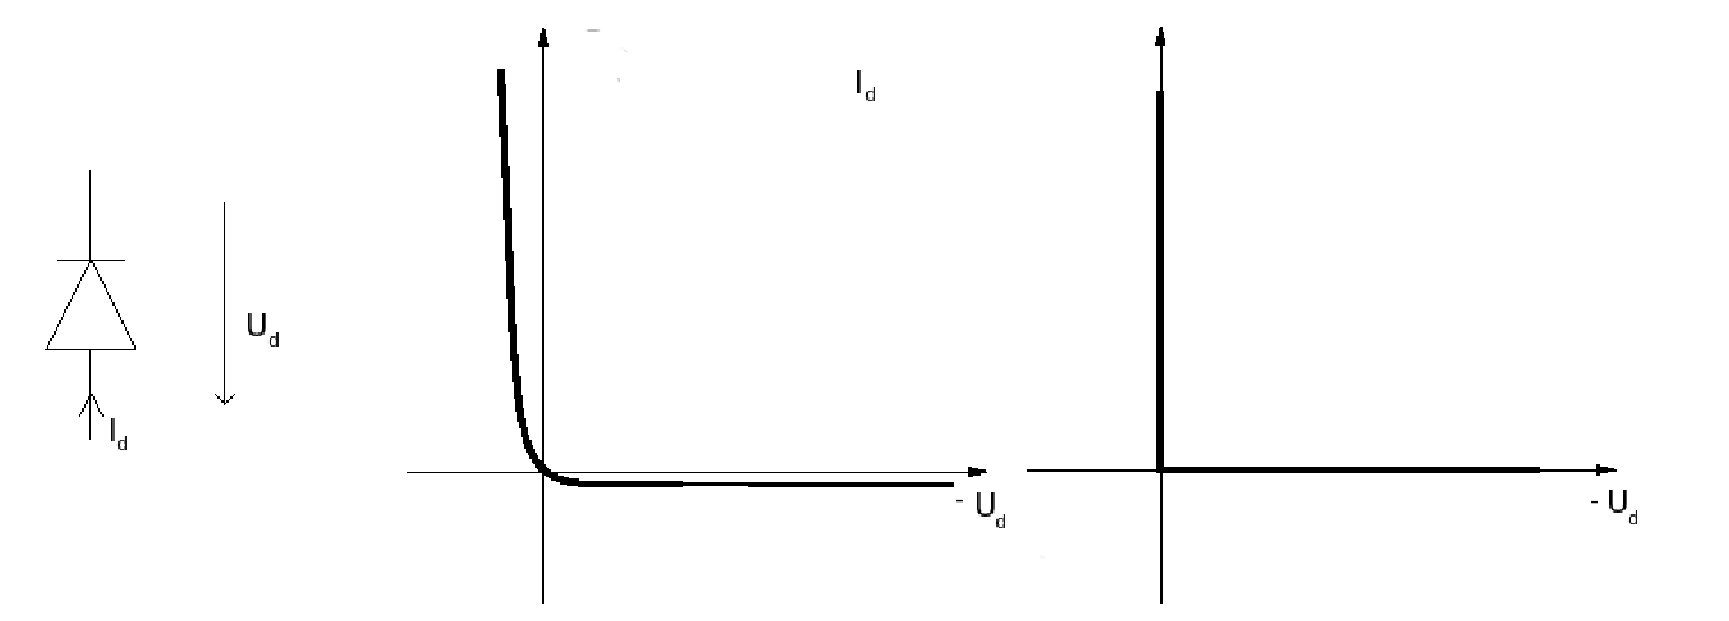
\includegraphics[width=100mm]{diode.eps}
  }
   \begin{block}{Branch Constitutive Equation of the diode:}
  \[ I_d =I_{s}(\exp{(-U_{D}/C)}-1)\]
  \end{block}
   \begin{block}{The complementary formulation:}
  \[0 \leq I_d \, \perp \, -U_{D} \geq 0\]
  \end{block}

}
\frame
{
  \frametitle{Ideal Transistor}
   \centerline{
  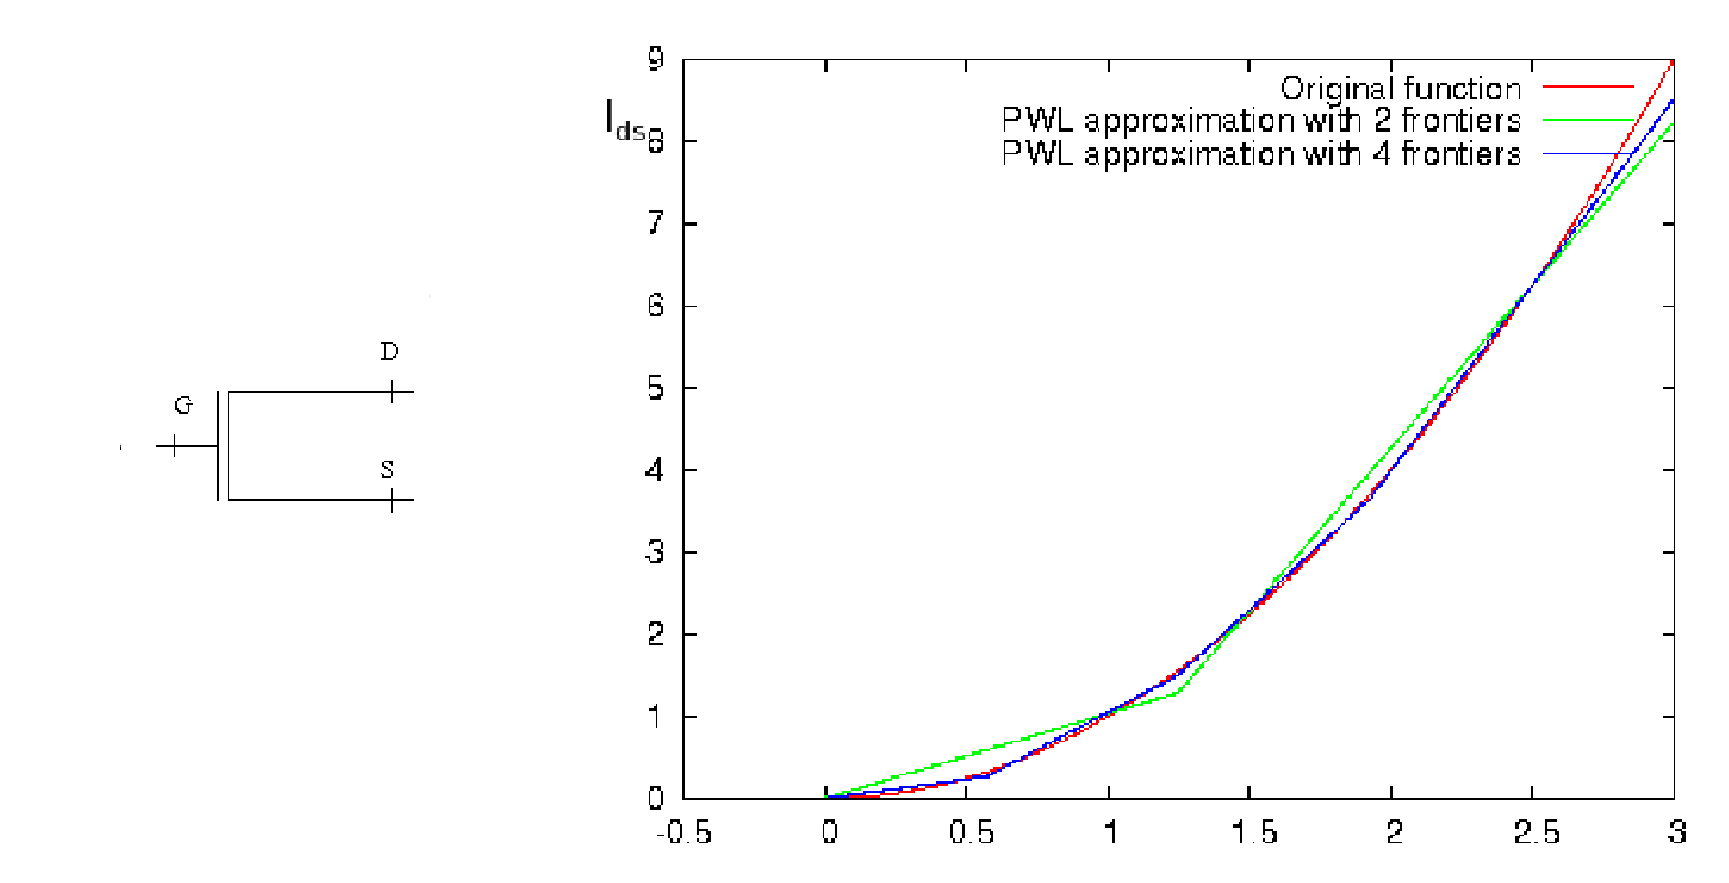
\includegraphics[width=100mm]{def2.eps}
  }
   \begin{block}{The complementary formulation:}
  \[ I_{d} = \left(\begin{array}{ccc}
  c_{1}&...&c_{10}\end{array}\right)\lambda \qquad  I_{d} = -I_{s}\]
  \[Y=A\left(\begin{array}{c}
  V_{d}\\
  V_{g}\\
  V_{s}\\\end{array}\right)+I\lambda + C\]
  \[0 \leq Y \, \perp \, \lambda \geq 0\]
  \end{block}

}

\section{Extend MNA for non-smooth components}

\frame
{
\frametitle{Extended MNA}
 It consists in replacing the Constitutive Equation of the non-smooth branch with the complementary
 formulation.

 \begin{block}{Unknowns}
 Before go ahead, the unknowns vector X is decomposed in:
\begin{itemize}
\item x which contains only the dynamic unknowns(currents in inductor and tensions from capacitor branches)
\item z which contains only the non dynamic unknowns(Voltage nodes,... ).
\end{itemize}
  \end{block}
  
 \begin{block}{A specific choice of unknowns yields the following system:}
 
 \begin{eqnarray}
x'=A_{2x}x +A_{2z}z +R \lambda +A_{2s}&\label{eq2}\\
0=B_{2x}x+B_{2z}z + B_{2\lambda}\lambda + B_{2s}&\label{eq3}\\
Y=D_{2x}x+D_{2z}z+D_{2\lambda}\lambda + D_{2s} &\label{eq4}\\
0 \leq Y \, \perp \, \lambda \geq 0&\label{eqperp}
\end{eqnarray}
\begin{itemize}
\item x which contains only the dynamic unknowns(currents in inductor and tensions from capacitor branches)
\item z which contains only the non dynamic unknowns(Voltage nodes,... ).
\end{itemize}

  \end{block}


}

%%% Local Variables: 
%%% mode: latex
%%% TeX-master: "main"
%%% End: 

\section{MLCS and MLCP}

\frame
{
\begin{block}{Mixed Linear Complementary System}
  Given the matrices   ${A_{x}} \in \RR^{n \times n}$, ${A_{z}} \in \RR^{n \times
  p}$, ${A_{v}} \in \RR^{n \times m}$, ${B_{x}} \in \RR^{p \times n}$, ${B_{z}} \in \RR^{p \times
  p}$, ${B_{v}} \in \RR^{p \times m}$, ${C_{x}} \in \RR^{m \times n}$, ${C_{z}} \in \RR^{m \times p}$,${C_{v}} \in \RR^{m \times m}$, and
  the vectors  $ {a} \in \RR^n$,$ {b}  \in \RR^p$,$ {c}  \in \RR^m$, the explicit MLCS denoted by
  $\mathrm{EMLCS}(A_{x},A_{z},A_{\lambda},B_{x},B_{z},B_{\lambda},C_{x},C_{z},C_{\lambda},a,b,c)$ consists in finding three vectors $ {x}
  \in \RR^n$, $ {z} \in \RR^p$ and  $ {\lambda} \in \RR^m$ such that
\begin{equation}\label{eq:mlcs2} 
  \begin{cases}
   x' = A_{x} x +A_{z} z +A_{\lambda} \lambda + a  \\
   0 = B_{x} x +B_{z} z + B_{\lambda} \lambda +b \\
   y=C_{x} x+ C_{z}z +C_{\lambda} \lambda +c\\
   {0} \le {\lambda} \perp     y  \ge {0}
  \end{cases}.
\end{equation}
\end{block}
The time discretization of a MLCS leads to :
\begin{block}{Mixed Linear Complementary Problem}
  Given the matrices  ${A} \in \RR^{n \times n}$, ${B} \in \RR^{m \times m}$, ${C} \in \RR^{n \times m}$, ${D} \in \RR^{m \times n}$, and the vectors  $ {a} \in \RR^n, {b} \in \RR^m$, the MLCP denoted by $\mathrm{MLCP}(A,B,C,D,a,b)$ consists in finding two vectors $ {y} \in \RR^n$ and  $ {\lambda} \in \RR^m$ such that
\begin{equation}
  \begin{cases}
    A u + C \lambda + a =0 \\
    y=Du +B \lambda +b\\
    {0} \le {\lambda} \perp    y   \ge {0}
  \end{cases} ie
  \begin{cases}
    M \left(\begin{array}{c}
    u\\ \lambda
    \end{array}\right)  +q = \left(\begin{array}{c}
    0\\ y
    \end{array}\right)\\
    {0} \le {\lambda} \perp    y   \ge {0}
  \end{cases}
\end{equation}
\end{block}
At each simulation step, a MLCP has to be solved. It is ensured using the SICONOS software.
}

\section{Solver MLCP}

\frame
{
\frametitle{MLCP to linear system}
\begin{block}{ Given a MLCP}
 \begin{equation}\label{eq:mlcp1}
 \begin{cases}
M \left(\begin{array}{c}
   U\\
   V
   \end{array}\right) + q = \left(\begin{array}{c}
   0\\
   W
   \end{array}\right) \\
      0 \le V \perp     W   \ge 0

      \end{cases}
\end{equation}


\end{block}

\begin{block}{A linear system}

Let $I_v$ and $I_w$, tow complementary subsets of $\{1,..,m\}$ and
looking for a solution such that : \\
\[
\begin{cases}
U_i=0 \textrm{ for } i \in I_v \\
 W_i=0 \textrm{ for } i \in I_w
\end{cases}
 \]




\[\textrm{Solve the linear system: }N \left(\begin{array}{c}
   U\\
   VW
   \end{array}\right) = -q   \textrm{   With   }
   \begin{cases}
   N_{.i}=M_{.i} \textrm{ for } i \in \{1..n\}\\
   N_{.i}=M_{.i} \textrm{ for } i-n \in I_w\\
   N_{.i}=-e_{i} \textrm{ for } i-n \in I_u
\end{cases}
\]
\[ \textrm { Solution if the complementarity hold: }
\begin{cases}
W_i \ge 0 \textrm{ for } i \in I_v  \\
U_i \ge 0 \textrm{ for } i \in I_w
\end{cases}
\]
An enumeratif algorithm consists in solving the $2^m$ cases.

\end{block}

}


\frame
{
\frametitle{A solver using the linear programming.\footnote{April 1983. An Enumerative Method for the Solution
of LCP By J.J. Judice and G. Mitra}}
\begin{block}{ Given a MLCP}
 

\begin{equation}\label{eq:mlcp1}
 \begin{cases}
M \left(\begin{array}{c}
   u\\
   \lambda
   \end{array}\right) + q = \left(\begin{array}{c}
   0\\
   y
   \end{array}\right) \\
      0 \le \lambda \perp     y   \ge 0

      \end{cases}
\end{equation}


\end{block}

\begin{block}{An interesting linear programming problem}
Let I and J, tow subsets of \{1,..,m\} with  $I \cap J = \emptyset$

\begin{equation}\label{eq:mlcp1}
\begin{cases}
M \left(\begin{array}{c}
   u\\
   \lambda
   \end{array}\right) + q = \left(\begin{array}{c}
   0\\
   y
   \end{array}\right)\\
\lambda_i = 0 \textrm{ for } i \in I \qquad \lambda_i \ge 0 \textrm{ for } i \notin I\\
y_j = 0 \textrm{ for } j \in J \qquad y_j \ge 0 \qquad j \notin J\\
\min{\sum_{i\notin I\cup J} \lambda_i + \sum_{j\notin I\cup J} y_j}
\end{cases}
\end{equation}
Tow cases:\\
\begin{itemize}
 \item[--] The minimization doesn't success, it means the constraints are not compatible, $\lambda_i =0 \textrm{ for } i \in I \qquad y_j=0 \textrm{ for } j\in J$ must be eliminated.\\
\item[--]Success, may the optimal point is a solution.
\end{itemize}

\end{block}

}

\frame
{
\frametitle{A branch and prune algorithm}
\[\left(\begin{array}{cccc}
4&0&0.2&0\\
0&2&0&0\\
1&0&0.2&0.5\\
0&0&0.5&0.2
 \end{array}\right) \left(\begin{array}{c}
 u_1\\
 u_2\\
 \lambda_1\\
 \lambda_2
 \end{array}\right) + \left(\begin{array}{c}
 -6\\
 -4\\
 -3\\
 2
 \end{array}\right) =  \left(\begin{array}{c}
 0\\
 0\\
 y_1\\
 y_2
 \end{array}\right) 
 \]
\begin{figure}[h]
\centerline{
 \scalebox{0.5}{
    \input{LP_step0.pstex_t}
 }
}
\end{figure}

}
\frame
{
\frametitle{A branch and prune algorithm}
\[\left(\begin{array}{cccc}
4&0&0.2&0\\
0&2&0&0\\
1&0&0.2&0.5\\
0&0&0.5&0.2
 \end{array}\right) \left(\begin{array}{c}
 u_1\\
 u_2\\
 \lambda_1\\
 \lambda_2
 \end{array}\right) + \left(\begin{array}{c}
 -6\\
 -4\\
 -3\\
 2
 \end{array}\right) =  \left(\begin{array}{c}
 0\\
 0\\
 y_1\\
 y_2
 \end{array}\right) 
 \]
\begin{figure}[h]
\centerline{
 \scalebox{0.5}{
    \input{LP_step1.pstex_t}
 }
}
\end{figure}

}
\frame
{
\frametitle{A branch and prune algorithm}
\[\left(\begin{array}{cccc}
4&0&0.2&0\\
0&2&0&0\\
1&0&0.2&0.5\\
0&0&0.5&0.2
 \end{array}\right) \left(\begin{array}{c}
 u_1\\
 u_2\\
 \lambda_1\\
 \lambda_2
 \end{array}\right) + \left(\begin{array}{c}
 -6\\
 -4\\
 -3\\
 2
 \end{array}\right) =  \left(\begin{array}{c}
 0\\
 0\\
 y_1\\
 y_2
 \end{array}\right) 
 \]
\begin{figure}[h]
\centerline{
 \scalebox{0.5}{
    \input{LP_step2.pstex_t}
 }
}
\end{figure}

}
\frame
{
\frametitle{A branch and prune algorithm}
\[\left(\begin{array}{cccc}
4&0&0.2&0\\
0&2&0&0\\
1&0&0.2&0.5\\
0&0&0.5&0.2
 \end{array}\right) \left(\begin{array}{c}
 u_1\\
 u_2\\
 \lambda_1\\
 \lambda_2
 \end{array}\right) + \left(\begin{array}{c}
 -6\\
 -4\\
 -3\\
 2
 \end{array}\right) =  \left(\begin{array}{c}
 0\\
 0\\
 y_1\\
 y_2
 \end{array}\right) 
 \]
\begin{figure}[h]
\centerline{
 \scalebox{0.5}{
    \input{LP_step3.pstex_t}
 }
}
\end{figure}

}

\frame
{
\frametitle{A reformulation using the Fischer-Burmeister function}
\begin{block}{ The Fischer-Burmeister function}
 
\[\phi (a,b) = a+b-\sqrt{a^2+b^2} \textrm{ and the merit function: } \psi (a,b) = \| \psi(a,b)\|^2 \]
Note that:
\[  0 \le a \perp     b   \ge 0 \Longleftrightarrow \phi (a,b) =0 \Longleftrightarrow (a,b) \textrm{is a
global minimum of } \psi \]
\end{block}

 Properties of theses functions: $\phi$ is strongly semi-smooth, $\psi$ is continuously defferentiable.

\begin{figure}[h]
\centerline{
 \scalebox{0.35}{
    \input{FischerB.pstex_t}
    \input{Psi.pstex_t}
 }
}
\end{figure}

 

}

\frame
{
\frametitle{A reformulation using the Fischer-Burmeister function}


\begin{block}{ MLCP reformulation}

\begin{equation}
  \begin{array}{cc}
   \begin{cases}
    A u + C v + a =0 \\
    {0} \le {v} \perp     Du +B v +b   \ge {0}
    \end{cases}&
   \begin{cases}
   \Phi :\mathbb{R}^{n+m} \longrightarrow \mathbb{R}^{n+m}\\
   \Phi(z)=\left(\begin{array}{c}
   \left(\begin{array}{cc}
   A&C
   \end{array}\right)z\\
   \phi(z_{n+1},(D_{1.}B_{1.})z)\\
   .\\
   .\\
   \phi(z_{n+m},(D_{m.}B_{m.})z)
   \end{array}\right)=0
    \end{cases}
  \end{array}
\end{equation}
This problem consists now in finding the global minimum of the merit function $\Psi(z)=\| \Phi(z)\|^2$.
 
\end{block}




}


\frame
{

\begin{equation}
  \begin{array}{c}
   \begin{cases}
    M1 \left(\begin{array}{c} u\\ v\end{array}\right)  + a =0 \\
    {0} \le {v} \perp     M2\left(\begin{array}{c} u\\ v\end{array}\right) +b   \ge {0}\\
    \textrm{ changement de variable : }
    N \left(\begin{array}{c} \tilde{u}\\ \tilde{v}\end{array}\right)=  \left(\begin{array}{c} u\\ v\end{array}\right)\\
    M1N \left(\begin{array}{c} \tilde{u}\\ \tilde{v}\end{array}\right)  + a =0 \\
    {0} \le {\left(N \left(\begin{array}{c} \tilde{u}\\ \tilde{v}\end{array}\right)\right)_{n..n+m}} \perp     M2N\left(\begin{array}{c} \tilde{u}\\ \tilde{v}\end{array}\right) +b   \ge {0}\\
    
    \end{cases}\\\\
   \begin{cases}
   \Phi :\mathbb{R}^{n+m} \longrightarrow \mathbb{R}^{n+m}\\
   \Phi \left(\begin{array}{c} \tilde{u}\\ \tilde{v}\end{array}\right)=\left(\begin{array}{c}
  
   M1N
   \left(\begin{array}{c} \tilde{u}\\ \tilde{v}\end{array}\right)_i\\
   \phi((N \left(\begin{array}{c} \tilde{u}\\ \tilde{v}\end{array}\right))_i,(M2N\left(\begin{array}{c} \tilde{u}\\ \tilde{v}\end{array}\right)_i)\\
   .\\
   .
   \end{array}\right)=0
    \end{cases}
  \end{array}
\end{equation}
  reste a choisir N pour condiionner $\left(\begin{array}{cc} 0&I\\A&C\\D&B\end{array}\right)$


 
 


}

\section{Cost of the automatic equation formulation}

\frame
{
\frametitle{Cost evaluation}
Let
\begin{itemize}
\item $N_{b}$ the number of branches.
\item $N_{n}$ the number of nodes.
\item N = max\{$N_{b},N_{n}$\}
\end{itemize}

\begin{block}{The costs of the automatic circuit equation formulation:}

\begin{itemize}
\item To parse the Netlist : It consists in reading and storing the Netlist. O(N).
\item A topological analysis to build the unknowns vector:
The Minimum Spanning Tree algorithm complexity is O(Nlog(N))
\item Stamping method:
Each component writes its contribution in the table equation. O(N).
\item Matrix product:
Multiplied two dense matrices costs O($N^{3}$).
\end{itemize}
\end{block}


}

\section{Simulation}

\frame
{
\frametitle{Diodes Bridge}

\begin{figure}[h]
\centerline{
 \scalebox{0.3}{
    \input{Bridge.pstex_t}
 }
}\end{figure}
\begin {figure}[h]
 \scalebox{0.5}{
%GNUPLOT: LaTeX picture with Postscript
\begin{picture}(0,0)%
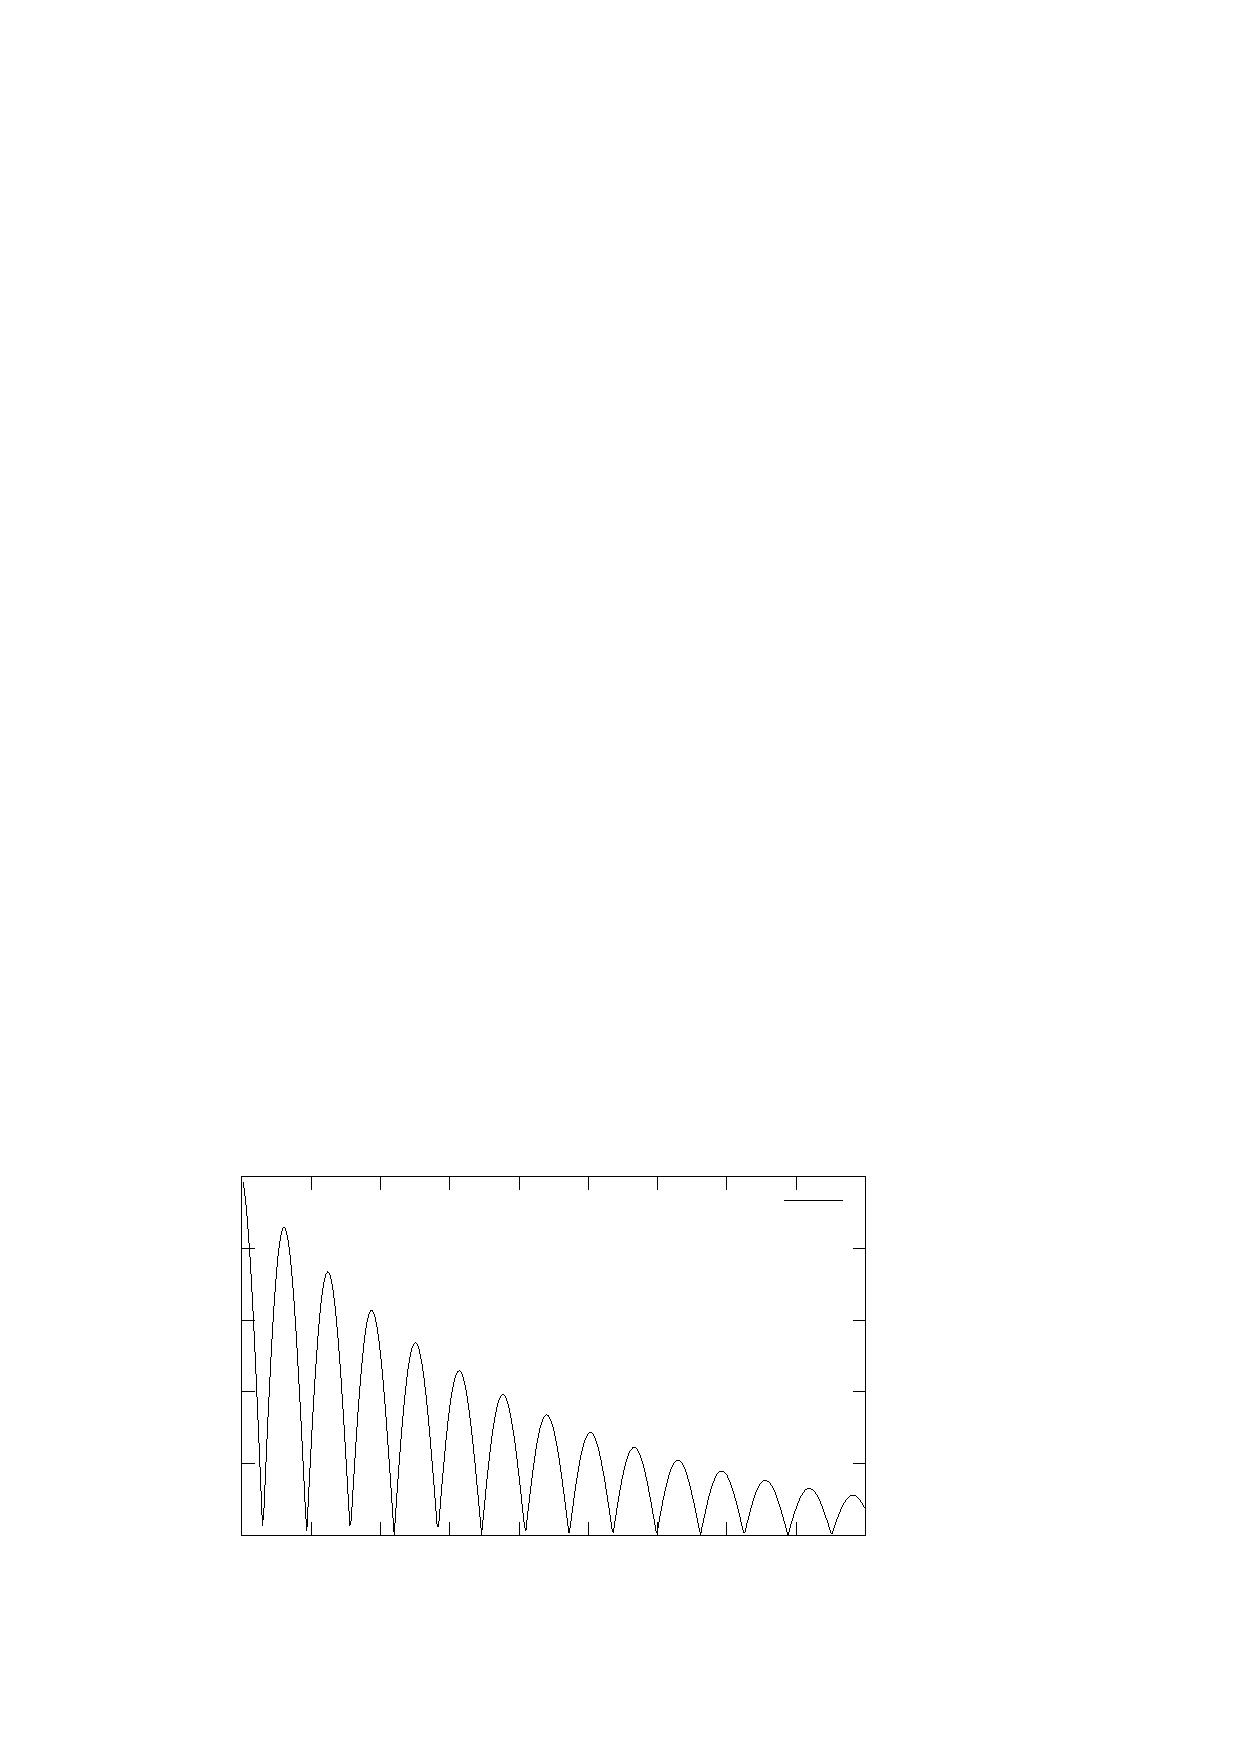
\includegraphics{diodes}%
\end{picture}%
\begingroup
\setlength{\unitlength}{0.0200bp}%
\begin{picture}(18000,10800)(0,0)%
\put(1925,1650){\makebox(0,0)[r]{\strut{} 0}}%
\put(1925,3370){\makebox(0,0)[r]{\strut{} 2}}%
\put(1925,5090){\makebox(0,0)[r]{\strut{} 4}}%
\put(1925,6810){\makebox(0,0)[r]{\strut{} 6}}%
\put(1925,8530){\makebox(0,0)[r]{\strut{} 8}}%
\put(1925,10250){\makebox(0,0)[r]{\strut{} 10}}%
\put(2200,1100){\makebox(0,0){\strut{} 0}}%
\put(3864,1100){\makebox(0,0){\strut{} 50}}%
\put(5528,1100){\makebox(0,0){\strut{} 100}}%
\put(7192,1100){\makebox(0,0){\strut{} 150}}%
\put(8856,1100){\makebox(0,0){\strut{} 200}}%
\put(10519,1100){\makebox(0,0){\strut{} 250}}%
\put(12183,1100){\makebox(0,0){\strut{} 300}}%
\put(13847,1100){\makebox(0,0){\strut{} 350}}%
\put(15511,1100){\makebox(0,0){\strut{} 400}}%
\put(17175,1100){\makebox(0,0){\strut{} 450}}%
\put(550,5950){\rotatebox{90}{\makebox(0,0){\strut{}U23}}}%
\put(9687,275){\makebox(0,0){\strut{}time e-5 s}}%
\put(14950,9675){\makebox(0,0)[r]{\strut{}'DiodeBridge.traj'}}%
\end{picture}%
\endgroup
\endinput

}
\end {figure} 

}
\frame
{
\frametitle{Buck converter}

\begin{figure}[h]
\centerline{
 \scalebox{0.5}{
    \input{buck.pstex_t}
 }
}\end{figure}
\begin {figure}[h]
 \scalebox{0.5}{
%GNUPLOT: LaTeX picture with Postscript
\begin{picture}(0,0)%
\includegraphics{Buck}%
\end{picture}%
\begingroup
\setlength{\unitlength}{0.0200bp}%
\begin{picture}(18000,10800)(0,0)%
\put(2200,1650){\makebox(0,0)[r]{\strut{}-0.7}}%
\put(2200,2725){\makebox(0,0)[r]{\strut{}-0.6}}%
\put(2200,3800){\makebox(0,0)[r]{\strut{}-0.5}}%
\put(2200,4875){\makebox(0,0)[r]{\strut{}-0.4}}%
\put(2200,5950){\makebox(0,0)[r]{\strut{}-0.3}}%
\put(2200,7025){\makebox(0,0)[r]{\strut{}-0.2}}%
\put(2200,8100){\makebox(0,0)[r]{\strut{}-0.1}}%
\put(2200,9175){\makebox(0,0)[r]{\strut{} 0}}%
\put(2200,10250){\makebox(0,0)[r]{\strut{} 0.1}}%
\put(2475,1100){\makebox(0,0){\strut{}   0}}%
\put(3945,1100){\makebox(0,0){\strut{}   2e-5}}%
\put(5415,1100){\makebox(0,0){\strut{}   4e-5}}%
\put(6885,1100){\makebox(0,0){\strut{}   6e-5}}%
\put(8355,1100){\makebox(0,0){\strut{}   8e-5}}%
\put(9825,1100){\makebox(0,0){\strut{}   1e-4}}%
\put(11295,1100){\makebox(0,0){\strut{}   1.2e-4}}%
\put(12765,1100){\makebox(0,0){\strut{}   1.4e-4}}%
\put(14235,1100){\makebox(0,0){\strut{}   1.6e-4}}%
\put(15705,1100){\makebox(0,0){\strut{}   1.8e-4}}%
\put(17175,1100){\makebox(0,0){\strut{}   2e-4}}%
\put(550,5950){\rotatebox{90}{\makebox(0,0){\strut{}Inductor current}}}%
\put(9825,275){\makebox(0,0){\strut{}time s}}%
\end{picture}%
\endgroup
\endinput

}
\caption{Buck converter simulation}
\end {figure} 

}
\section{Conclusion}

\frame
{
\begin{block}{The actual software version is able to parse and simulate a Netlist composed of:}
\begin{itemize}
\item Non constant sources.
\item Linear components : resistor, capacitor, inductance.
\item Non smooth components : Diode, Transistor, comparator.
\end{itemize}
\end{block}
\pause
\begin{block}{Perspectives}
\begin{itemize}
\item Topological analysis to index reduction of the DAE.
\item Multigrid algorithm: use a more simple picewise linear approximation.
\item Forecast active set: use a local piecewise linear approximation to solve a smaller MLCP.
\item Mixed Newton/MLCP simulator.
\item Specific electrical heuristics.
\item Improve the component model.
\end{itemize}
\end{block}

}



\def\newblock{}

\end{document}
%%% Local Variables: 
%%% mode: latex
%%% TeX-master: main
%%% End: 
